\documentclass[a4paper, 12pt]{article}
\usepackage{cmap}
\usepackage{mathtext}
\usepackage{amsmath,amssymb}
\usepackage[T2A]{fontenc}
\usepackage[utf8]{inputenc}
\usepackage[english, russian]{babel}
\usepackage{bmstu-lab}
\usepackage{mathtools}
\usepackage{amsmath,amssymb} % AMS
\usepackage{graphicx} % Для вставки рисунков
\usepackage{lipsum} % lorem ipsum
\usepackage{array,tabularx,tabulary,booktabs} % Таблицы
\usepackage{multirow} % Слияние строк в таблице
\usepackage{diagbox}


\begin{document}
\graphicspath{{images/}{images2/}} % папки с картинками

\worknumber{2}
\variant{10}
\workname{Рисунки и таблицы}
\discipline{Автоматизация процессов разработки научно-технической документации}
\group{ИУ6-65Б}
\date{27.02.21}
\author{А.Н.Золкин}
\tutor[Преподаватель]{Т.А.Ким}
\bmstutitlelab

\newpage
\begin{center}
  \begin{tabular}{|l|r|c|}
    \hline
    $\times$ &            & $\bigcirc$ \\
    \hline
    $\times$ & $\bigcirc$ &            \\
    \hline
    $\times$ & $\times$   & $\bigcirc$ \\
    \hline
  \end{tabular}
\end{center}
\newpage
\begin{figure}[t]
  \centering
  
\includegraphics[scale=0.18]{image_1}
  \caption{Суровая правда}
\end{figure}
\begin{figure}[b]
  \centering
  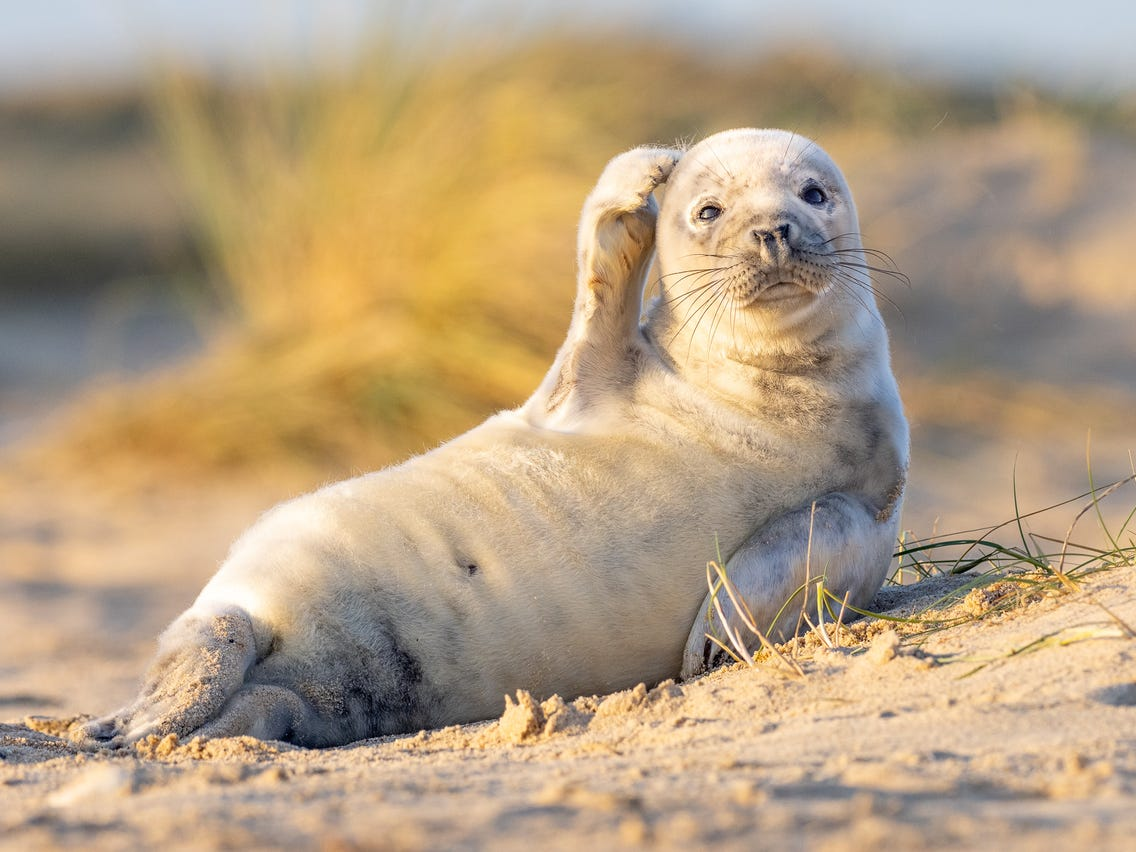
\includegraphics[scale=0.20]{image_2}
  \caption{Задает стандарт фотогеничности}
\end{figure}
\lipsum[1-3]
\begin{figure}[h]
  \centering
  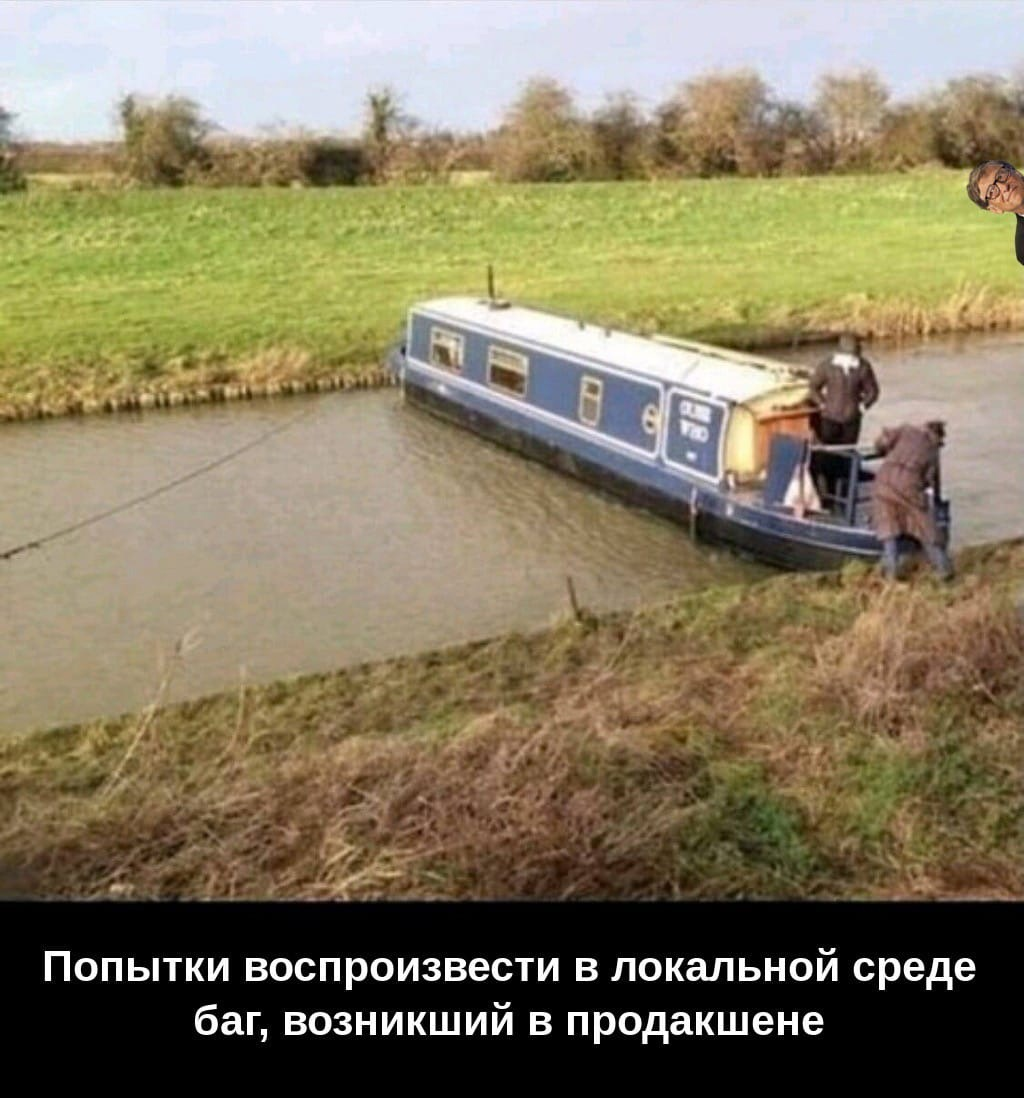
\includegraphics[scale=0.20]{image_3}
  \caption{Разработка в ногу со временем}
\end{figure}

\newpage
\begin{table}[h]
  \begin{center}
    \begin{tabular}{ ||c c c c c c c c c c c c c c c c|| }
      \hline
      \hline
       &  &                        &  &  &  &  &  &                        &  &  &  &  &  &   & \\
      \cline{3-10}
       &  & \multicolumn{8}{|c|}{} &  &  &  &  &  &                                             \\
      \cline{3-10}
       &  &                        &  &  &  &  &  &                        &  &  &  &  &  &   & \\
       &  &                        &  &  &  &  &  &                        &  &  &  &  &  &   & \\
       &  &                        &  &  &  &  &  &                        &  &  &  &  &  &   & \\
       &  &                        &  &  &  &  &  &                        &  &  &  &  &  &   & \\
       &  &                        &  &  &  &  &  &                        &  &  &  &  &  &   & \\
       &  &                        &  &  &  &  &  &                        &  &  &  &  &  &   & \\
       &  &                        &  &  &  &  &  &                        &  &  &  &  &  &   & \\
       &  &                        &  &  &  &  &  &                        &  &  &  &  &  &   & \\
      \cline{9-10}
       &  &                        &  &  &  &  &  & \multicolumn{2}{|c|}{} &  &  &  &  &  &     \\
      \cline{9-10}
       &  &                        &  &  &  &  &  &                        &  &  &  &  &  &   & \\
       &  &                        &  &  &  &  &  &                        &  &  &  &  &  &   & \\
       &  &                        &  &  &  &  &  &                        &  &  &  &  &  &   & \\
      \cline{3-5}
      \hline
      \hline
    \end{tabular}
  \end{center}
\end{table}

\newpage
\begin{center}
  \begin{tabular}{|c|c|c|} \hline
    \multirow{2}{*}{\backslashbox{2}{1}}
      & \multicolumn{2}{c|}{2}      \\
    \cline{2-3}
      & 22                     & 23 \\\hline
    1 & 121                    & 5  \\\hline
  \end{tabular}
\end{center}
\end{document}
